\documentclass[12pt,a4paper,twoside]{article}
\usepackage{labor}
\begin{document}

%fill for cover and header creation
\newcommand\laboratorynumber{2}
\title{Refraktometer}
\newcommand\supervisor{Ditlbacher, Harald}
\newcommand\groupnumber{42}

\newcommand\participantonelastname{Eisner}
\newcommand\participantonefirstname{Nico}
\newcommand\participantoneid{12214121}
\newcommand\participanttwolastname{Waldl}
\newcommand\participanttwofirstname{Philip}
\newcommand\participanttwoid{12214120}
\author{\participantonelastname \ \& \participanttwolastname}

\newcommand\degreeid{UB 033 678}
\newcommand\semester{23WS}
\date{24.11.2023}

%select correct course title
%\newcommand\coursetitle{Einführung in die \\ physikalischen Messmethoden}
%\newcommand\coursetitle{Laborübungen 1: \\ Mechanik und Wärme}
\newcommand\coursetitle{Laborübungen 2: \\ Elektrizität, Magnetismus, Optik}
%\newcommand\coursetitle{Fortgeschrittenen Praktikum 1: \\ Technische Physik}
%\newcommand\coursetitle{Fortgeschrittenen Praktikum 2: \\ Allgemeine Physik}

%\begin{titlepage}
   \begin{center}
       \begin{figure}[H]
            \begin{minipage}[h]{30mm}
                \centerline{
\includegraphics[height=15mm]{cover_nudes/tugraz.png}}
            \end{minipage}
            \hfill
            \begin{minipage}[h]{30mm}
                \centerline{
\includegraphics[height=15mm]{cover_nudes/nawi_graz.png}}
            \end{minipage}
            \hfill
            \begin{minipage}[h]{30mm}
                \centerline{
\includegraphics[height=15mm]{cover_nudes/uni-graz.png}}
            \end{minipage}
        \end{figure}
        
        \large{\emph{Institut für Experimentalphysik der Technischen Universität Graz \\
        \& Institut für Physik der Universität Graz}} \\
        \vspace{5mm}
        
        {\Huge \textbf{\coursetitle}}
        \vspace{5mm}
        
        {\huge \laboratorynumber: \thetitle}
    \end{center}
    
    \vfill
    
    \begin{table}[H]
        \LARGE
        \centering
        \begin{tabular}{r l}
            Betreuer:       & \supervisor \\
            Gruppennummer:  & \groupnumber \\
            \\
            Name:           & \participantonelastname, \participantonefirstname \\
            Matrikelnummer: & \participantoneid \\
            Name:           & \participanttwolastname, \participanttwofirstname \\
            Matrikelnummer: & \participanttwoid \\
            \\
            Kennzahl:       & \degreeid \\
            Datum:          & \semester \ | \thedate
        \end{tabular}
    \end{table}
    \vspace{4cm}
\end{titlepage}
\clearpage
\setcounter{page}{1}

%\maketitle %short title alternative

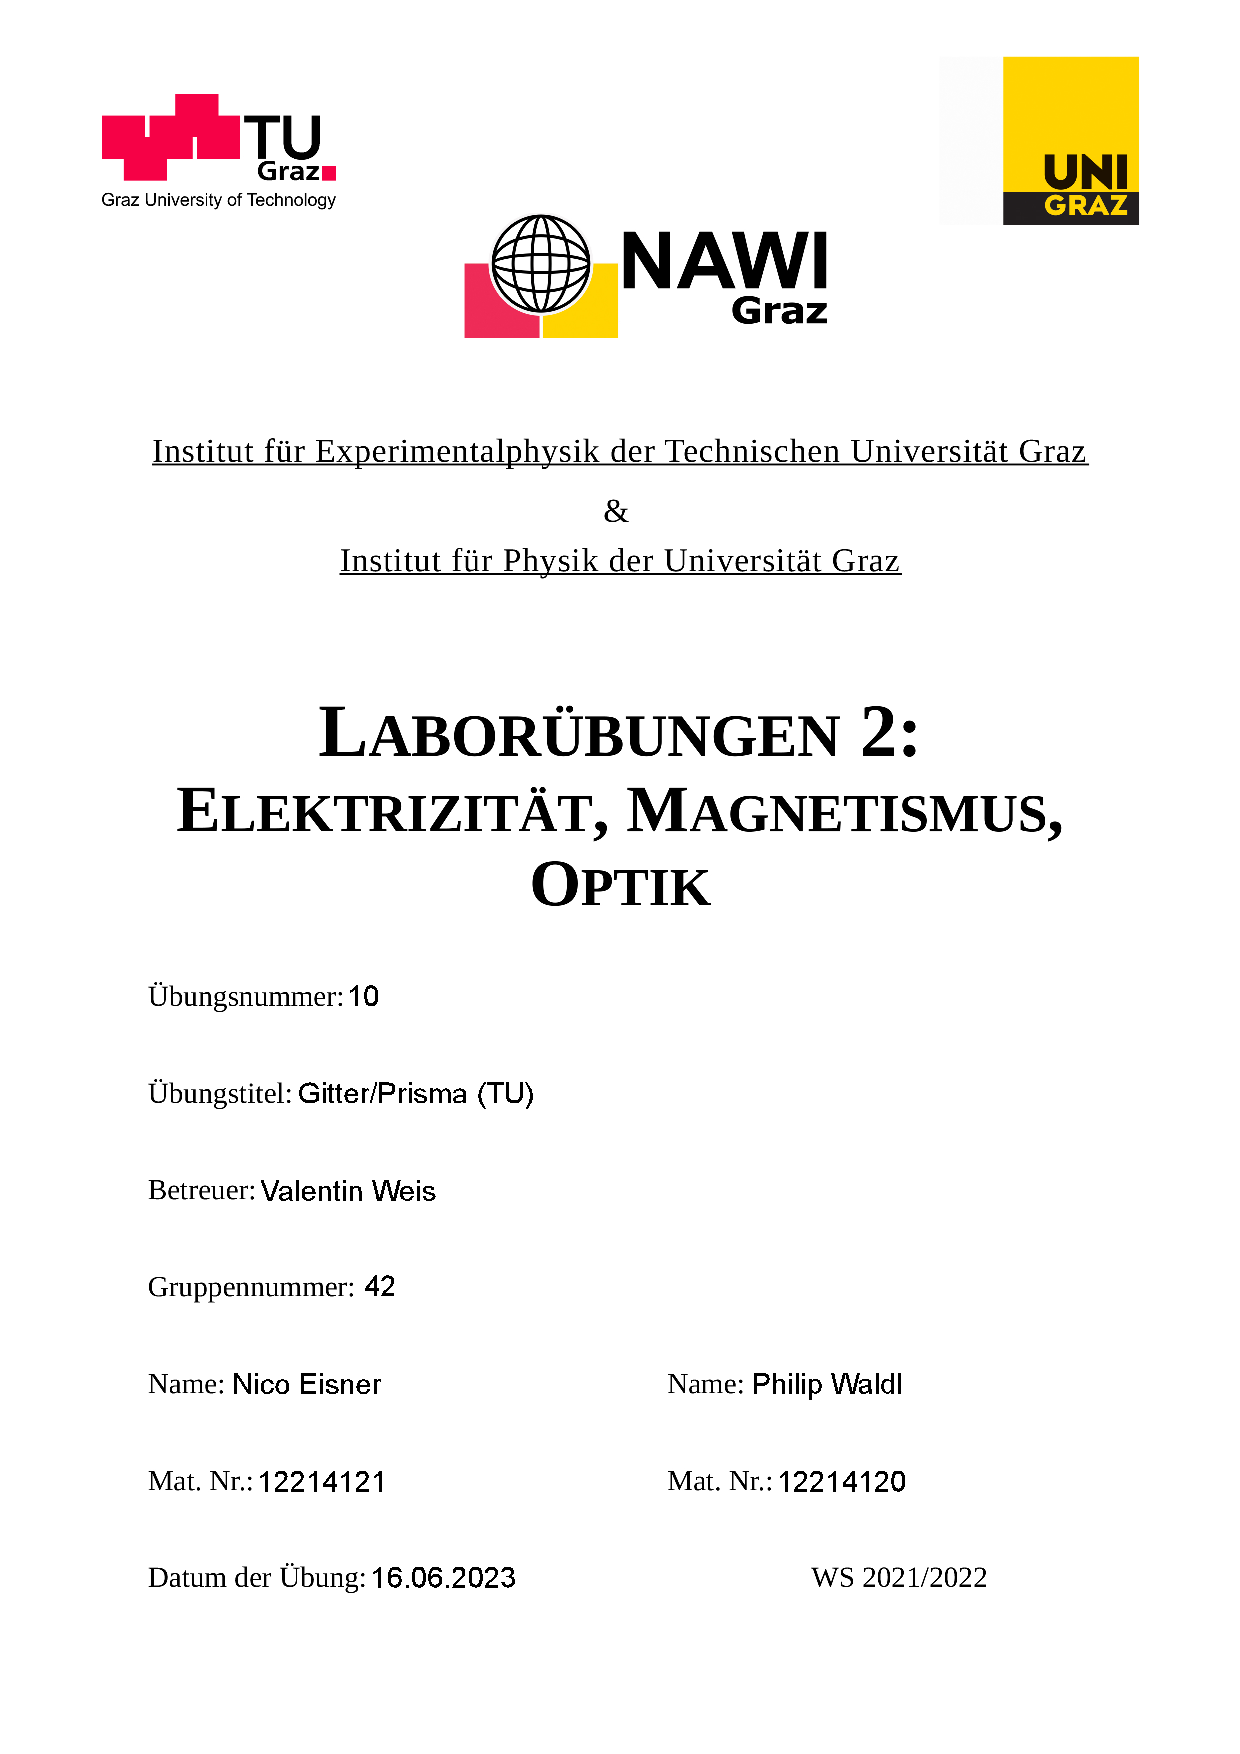
\includepdf[pages={1}]{../Deckblätter/Deckblatt_Gitter.pdf}

\tableofcontents
\newpage

\section{Aufgabenstellung} %jo beschreibn wos gmocht host ------------------------------
Das Experiment Grenzflächen / Refraktometer besteht aus zwei Teilversuchen. 
\\
Im Ersten, wird mit einem Reflexions-Refraktometer an einer Grenzfläche zweier Medien das Reflexionsvermögen gemessen. 
Dabei ist die Messung von Medium 1 zu Medium 2 und umgekehrt durchzuführen. 
\\
Im zweiten Teilversuch werden mit einem Abbe-Refraktometer die Brechungsindizes zweier verschiedener Flüssigkeiten bestimmt. 
\\
\\
Alle Informationen und Methodiken wurden uns von der Technischen Universität bereitgestellt \cite{teachcenter2}. 

\section{Voraussetzungen \& Grundlagen} %Grundlagen erklären, Formeln mit erklärung
Um mit dem Experiment zu beginnen, gilt es erst einige Grundlagen zu kennen. 
\\
\\
Um das Reflexionsvermögen $R$ zu bestimmen, benötigt man die Detektorspannungen bei direktem Einfall des Laserstrahles $U_0$ sowie bei reflektiertem Einfall des Laserstrahles durch die Medien $U_R$. 
Wenn der Laserstrahl nicht auf den Detektor trifft, ist dennoch eine Spannung zu messen. Diese Spannung $U_D$ ist das Dunkelstromrauschen des Detektors und der Photostrom der Umgebungsbeleuchtung. 
\\
Um nun das Reflexionsvermögen $R$ zu berechnen, benötigt man die Intensität $I$ welche vom Detektor ausgebeben wird. 
Dabei ist die Refernzintensität $I_0 \varpropto U_0 - U_D$ und die Reflexionsintensität $I_R \varpropto U_R - U_D$. 
Daraus lässt sich das Reflexionsvermögen $R$ mit Unsicherheit $\Delta R$ berechnen. 

\begin{equation}
    \label{eq:Reflexionsvermögen}
    \centerline{$R=\frac{I_R}{I_0}$ \\ $\Delta R = \vert \frac{\partial R}{\partial I_R} * \Delta I_R \vert + \vert \frac{\partial R}{\partial I_0} * \Delta I_0 \vert$}
\end{equation}

\noindent
Im Ersten Teil wird das Reflexionsvermögen bei einem p-Polarisierten und einen s-Polarisierten Laserstrahl gemessen. 
\\
Ein p-Polarisierter Laserstrahl ist parallel zur Einfallsebene polarisiert und ein s-Polarisierter senkrecht zur Einfallsebene. 
P-Polarisation lässt sich durch den Brewsterwinkel bestimmen. Dazu dreht man den Polarisator so lange, bis der reflektierte Strahl ab einen gewissen Winkel verschwindet. 
Um 90° verschoben ist der Laserstrahl s-Polarisiert. 

\begin{figure}[H]
    \centering
    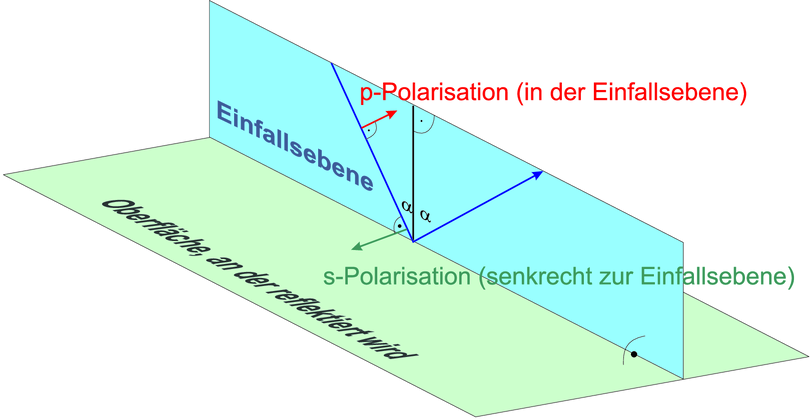
\includegraphics[width=0.6\linewidth]{nudes/sp pol.png}
    \caption{Darstellung eines p-Polarisierten und s-Polarisierten Lichtstrahles. \cite{Polarisation}}
    \label{fig:s-p-Polarisiert}
\end{figure}

\noindent
Um den Brechungswinkel $\beta$ zu bestimmen, benötigt man das Brechungsgesetz von Snellius. Dafür benötigt man die Brechungsindizes $n$ der Medien sowie den einfallenden Winkel $\alpha$. 

\begin{equation}
    \label{eq:Snellius}
    \centerline{$n_1 * sin(\alpha) = n_2 * sin(\beta)$ \\ $\Delta \beta = \vert \frac{\partial \beta}{\partial \alpha} * \Delta \alpha \vert + \vert \frac{\partial \beta}{\partial n_1} * \Delta n_1 \vert + \vert \frac{\partial \beta}{\partial n_2} * \Delta n_2 \vert$}
\end{equation}

\noindent
Für die Bestimmung der Brechungsindizes $n$ mit einem Abbe-Refraktometer benötigt man die im Okular abgelesene Werte des Brechungsindex $n_D$ und Brix sowie den Kompensatorwert. 
Mithilfe des Nomogrammes wird die mittlere Dispersion $n_f-n_D$ bestimmt. 

\begin{figure}[H]
    \centering
    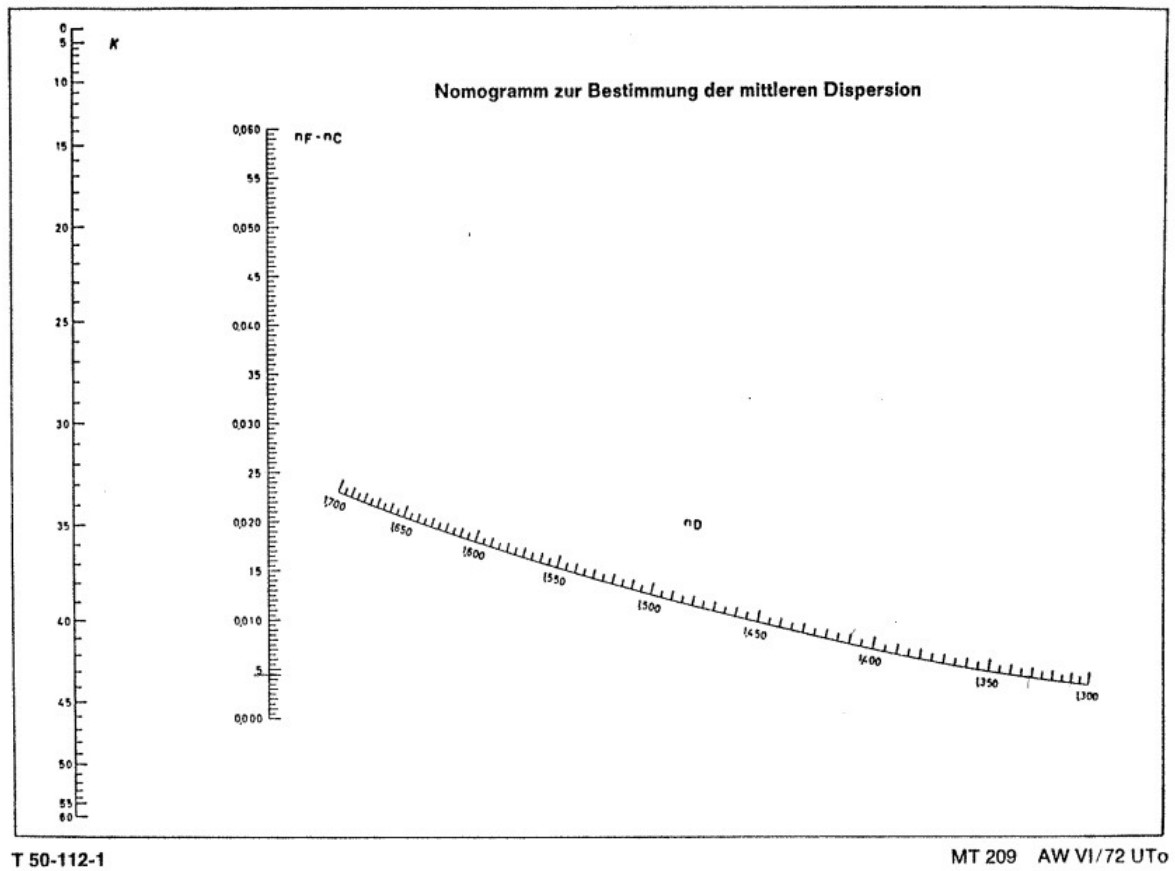
\includegraphics[width=0.6\linewidth]{nudes/nomogramm.jpg}
    \caption{Nomogramm zur bestimmung der mittleren Dispersion $n_f-n_D$. Entnommen aus Skript Fresnel Seite 14. \cite{teachcenter2}}
    \label{fig:nomogramm}
\end{figure}

\section{Versuchsanordnung} %mit skizze kurz beschreiben ------------------------------
Der Versuch ist wiefolgt aufgebaut. 

\begin{figure}[H]
    \centering
    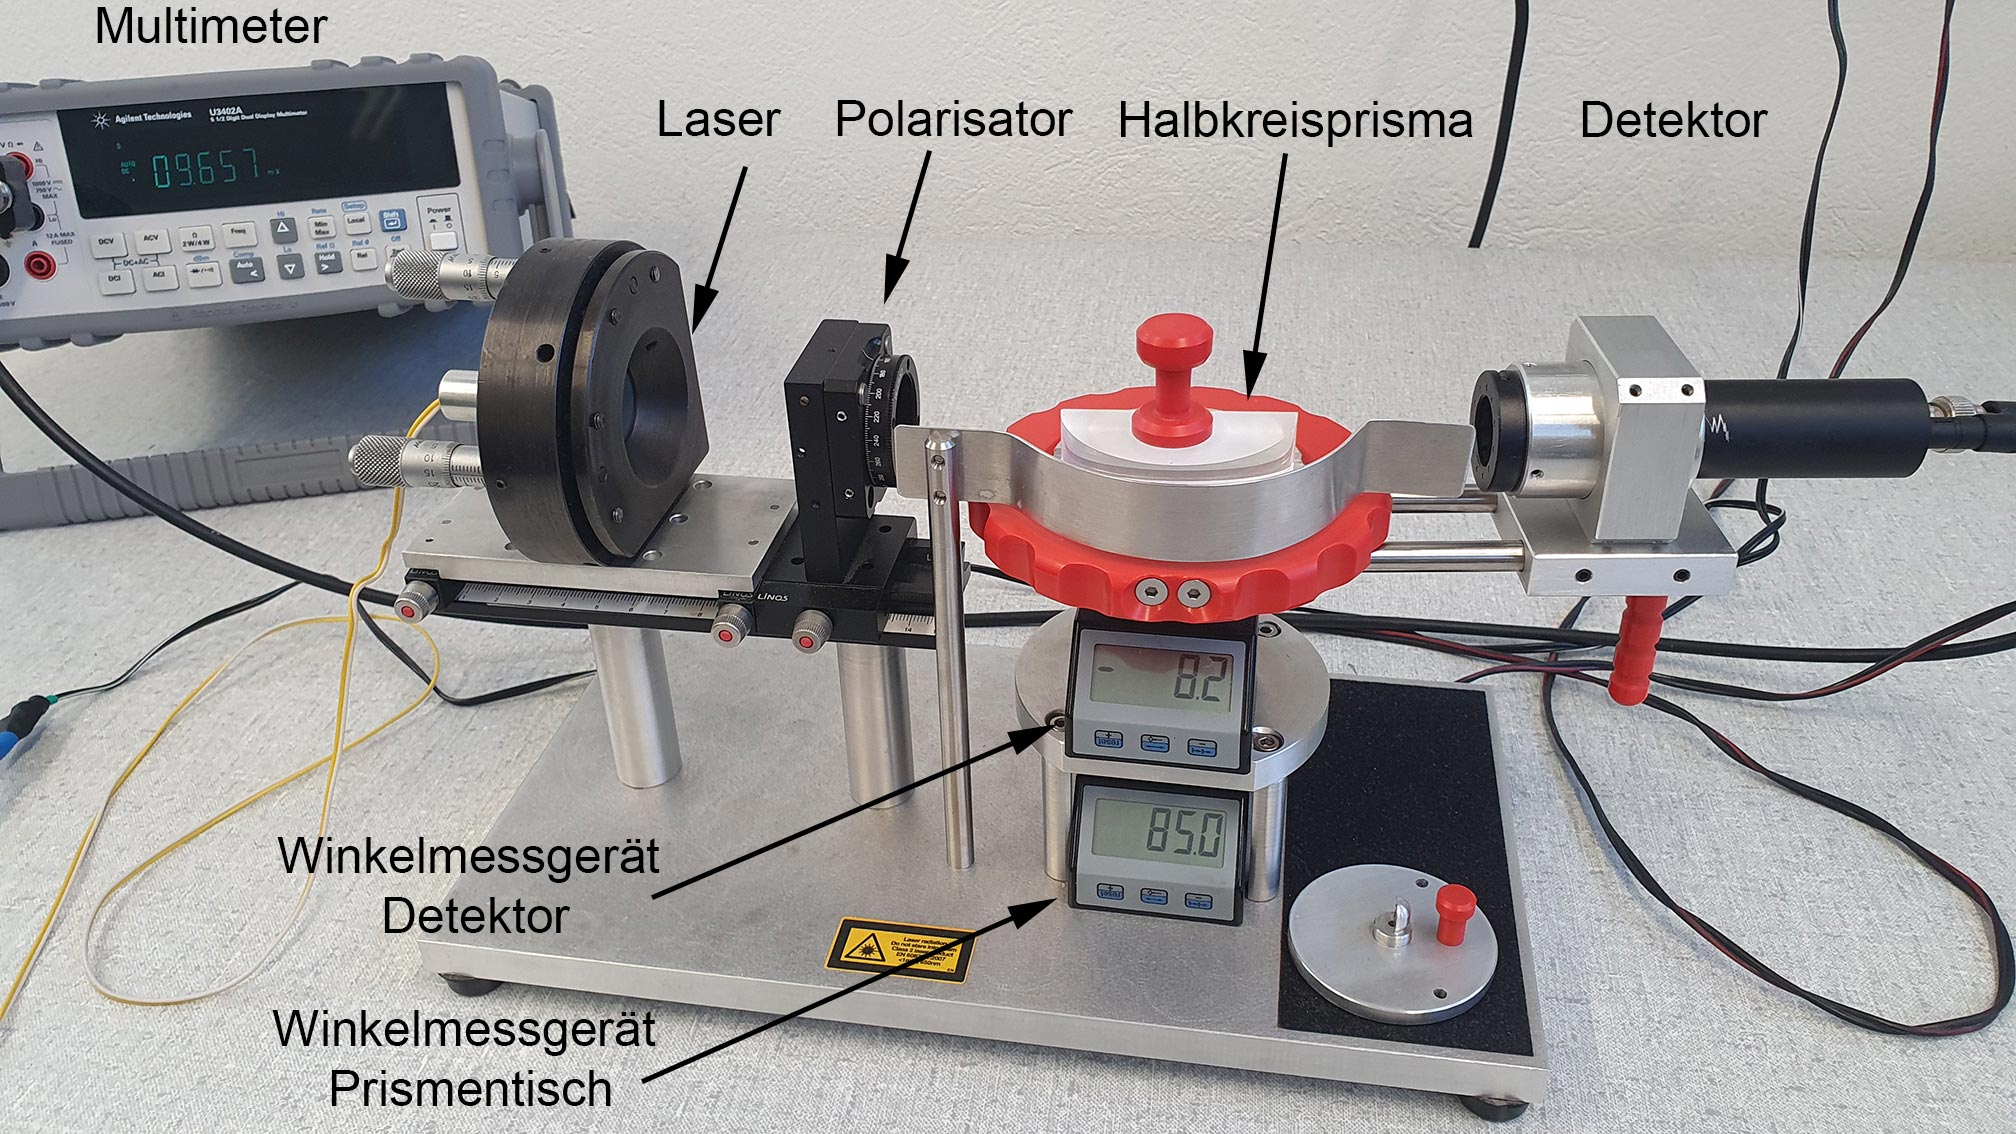
\includegraphics[width=0.6\linewidth]{nudes/Aufbau.jpg}
    \caption{Aufbau des Versuches Refexions-Refraktometer}
    \label{fig:aufbau}
\end{figure}

\noindent
Ein Laser sendet Lichtstrahlen durch einen Polarisator, welche auf einen Halbkreisprisma treffen. Dort werden die Lichtstrahlen gebrochen und es entsteht ein refkektierender Strahl und ein gebrochener Strahl. 
Dieser Strahl wird von einem Detektor gemessen und als Spannung am Multimeter dargestellt. 

\begin{figure}[H]
    \centering
    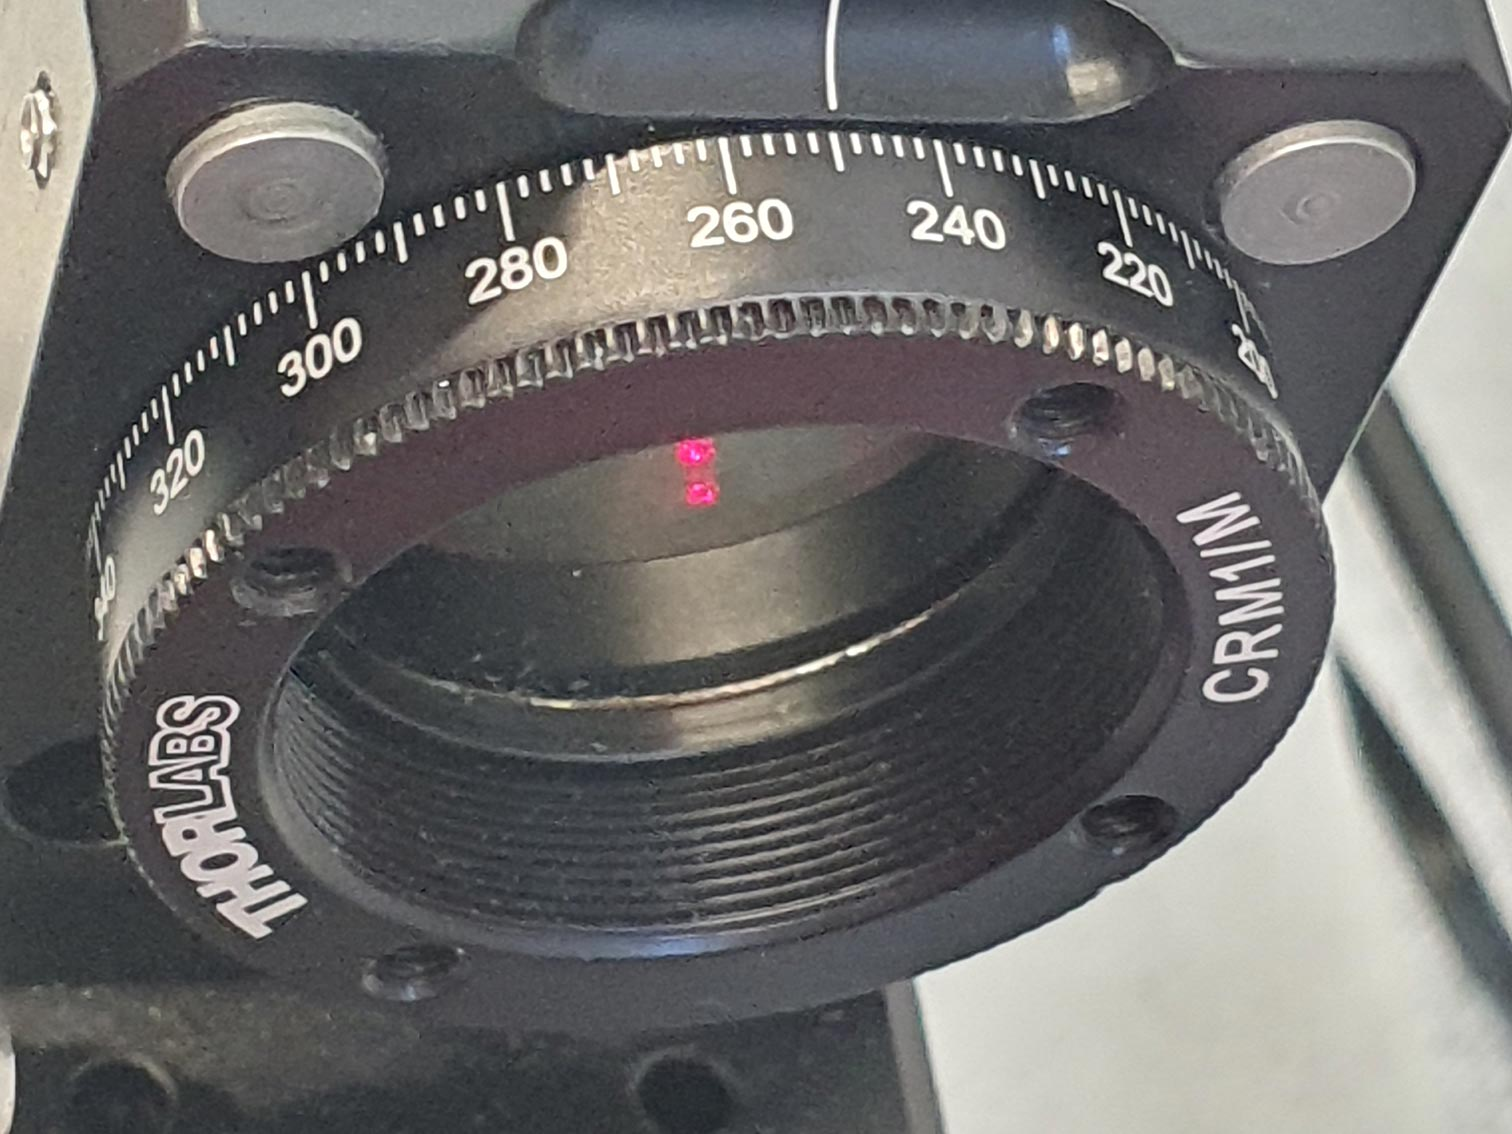
\includegraphics[width=0.4\linewidth]{nudes/Polarisator.jpg}
    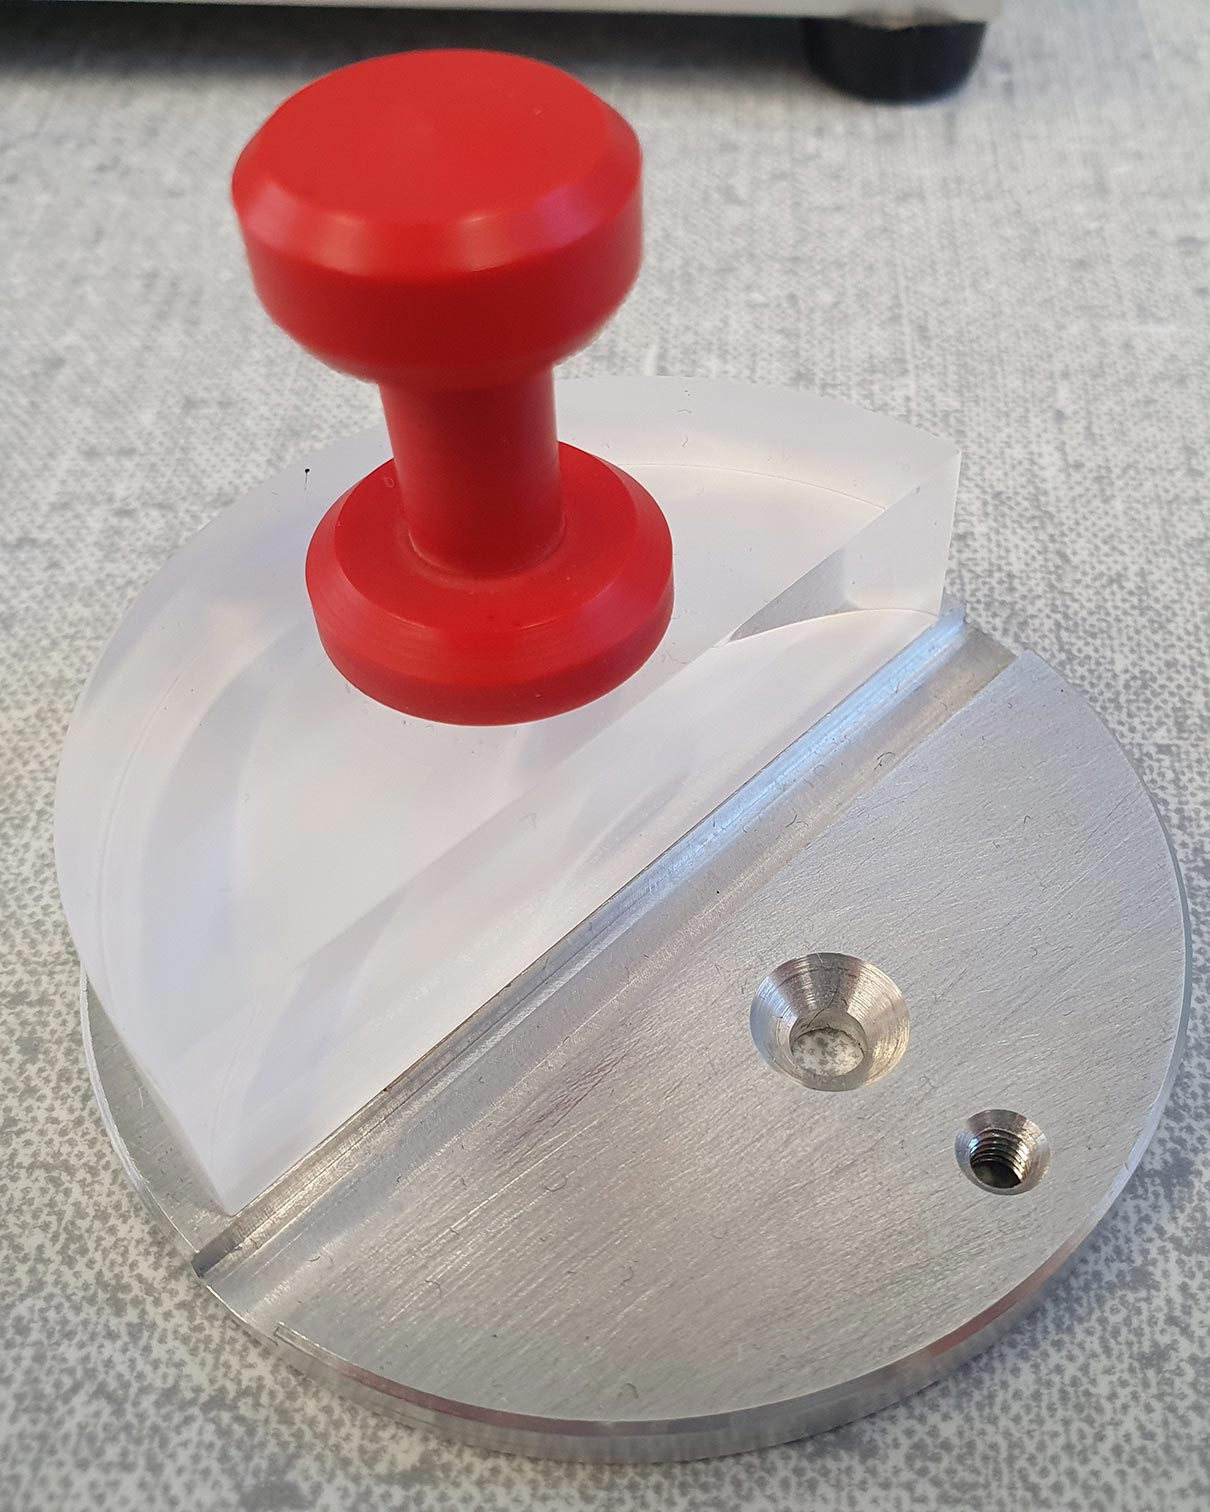
\includegraphics[width=0.4\linewidth]{nudes/halbkreisprisma.jpg}
    \caption{Polarisator mit Winkelskala (rechts) und Halbkreisprisma (links). }
    \label{fig:Polarisator und prisma}
\end{figure}

\noindent
Durch Drehen des Polarisators lässt sich der Lichtstrahl in p-Polarisiertes oder s-Polarisiertes Licht polarisieren. 
Dabei wird der Prisma gedreht und die Blende des Detektors wird geschlossen, um den Detektor genau auf den reflektierenden Strahl zu lenken. 
\\
\\
Bei dem Abbe-Refraktometer wird die zu bestimmende Flüssigkeit auf den Prisma gegeben. Durch die Beleuchtung mit weißem Licht kommt es zu einer Farbaufspaltung. 
Durch Ausgleichen dieser Aufspaltung mit Kompenstorprismen wird der Brechungsindex und Brix abgelesen. 

\begin{figure}[H]
    \centering
    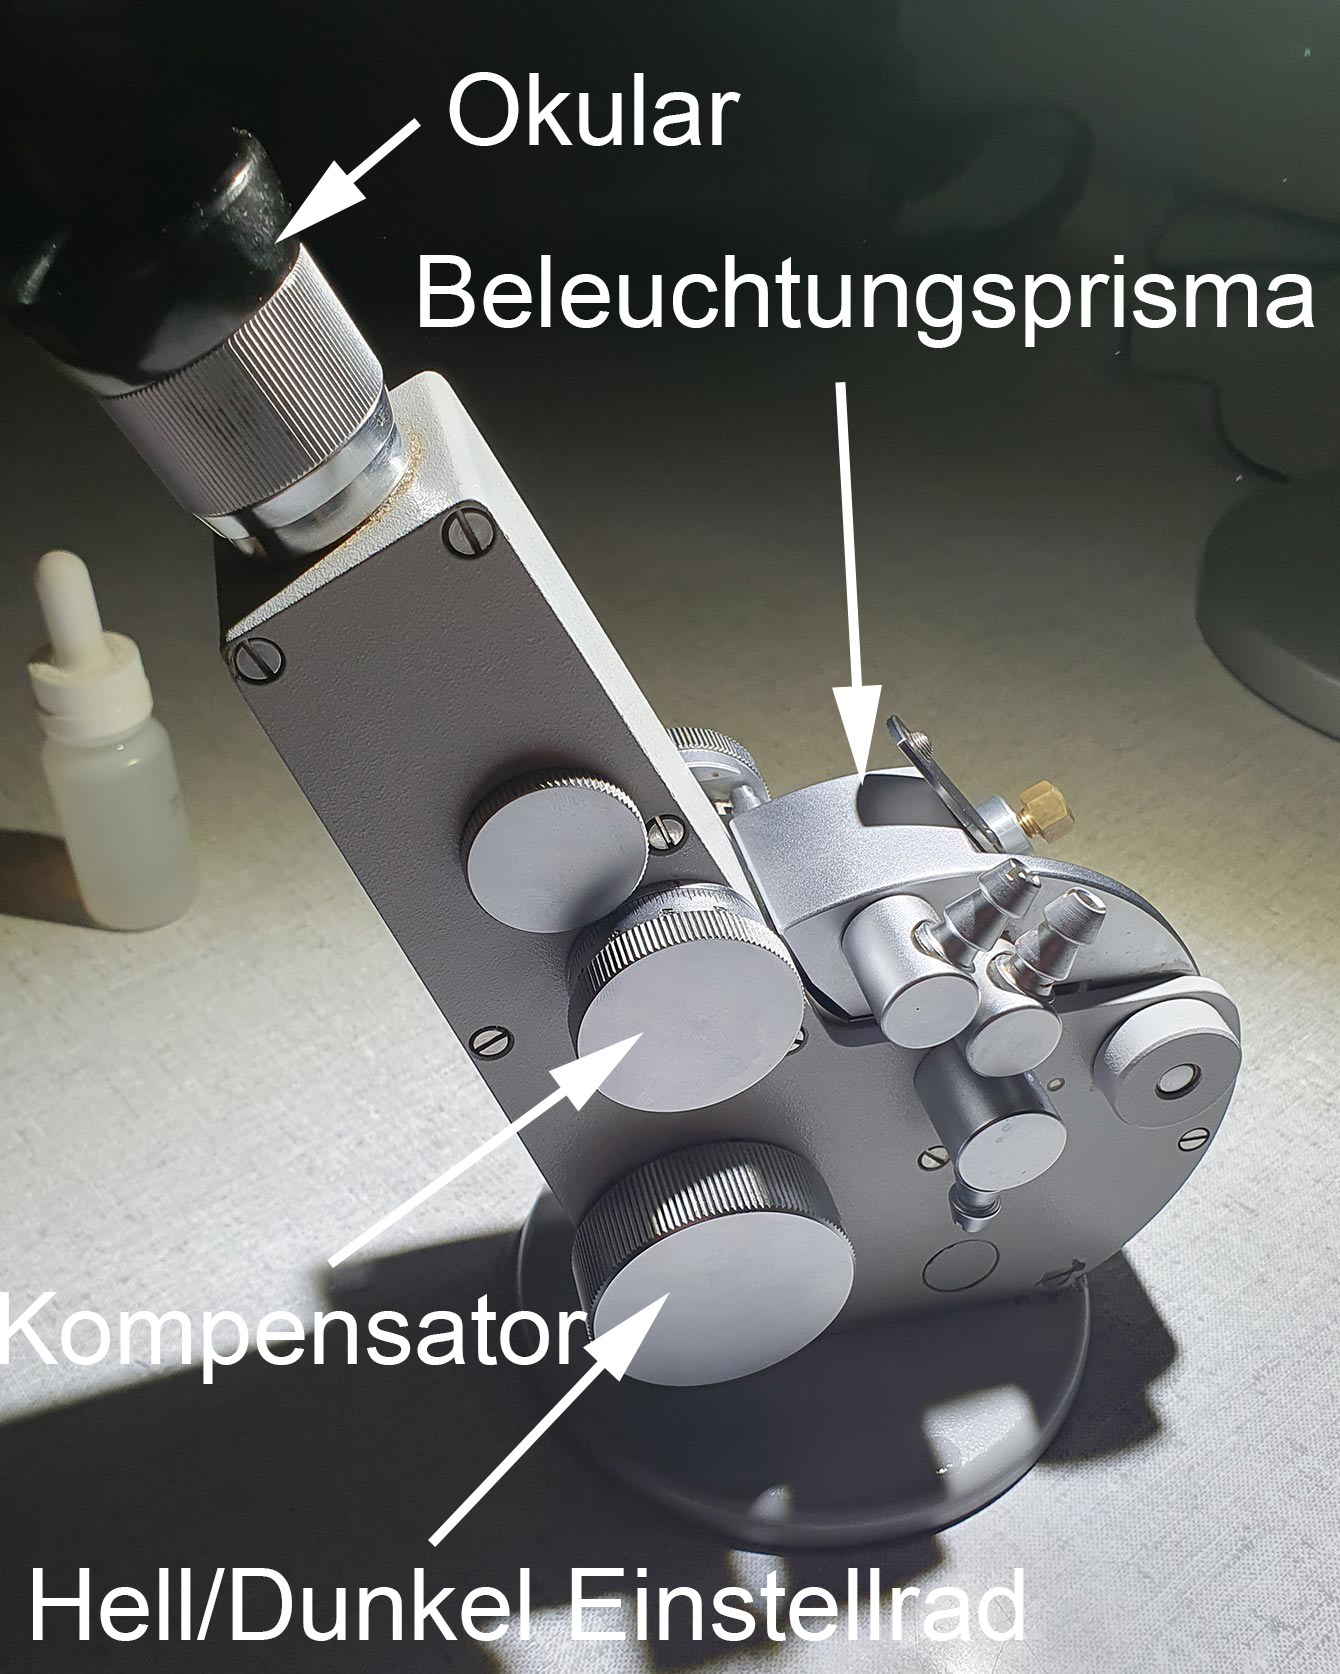
\includegraphics[width=0.4\linewidth]{nudes/abbe.jpg}
    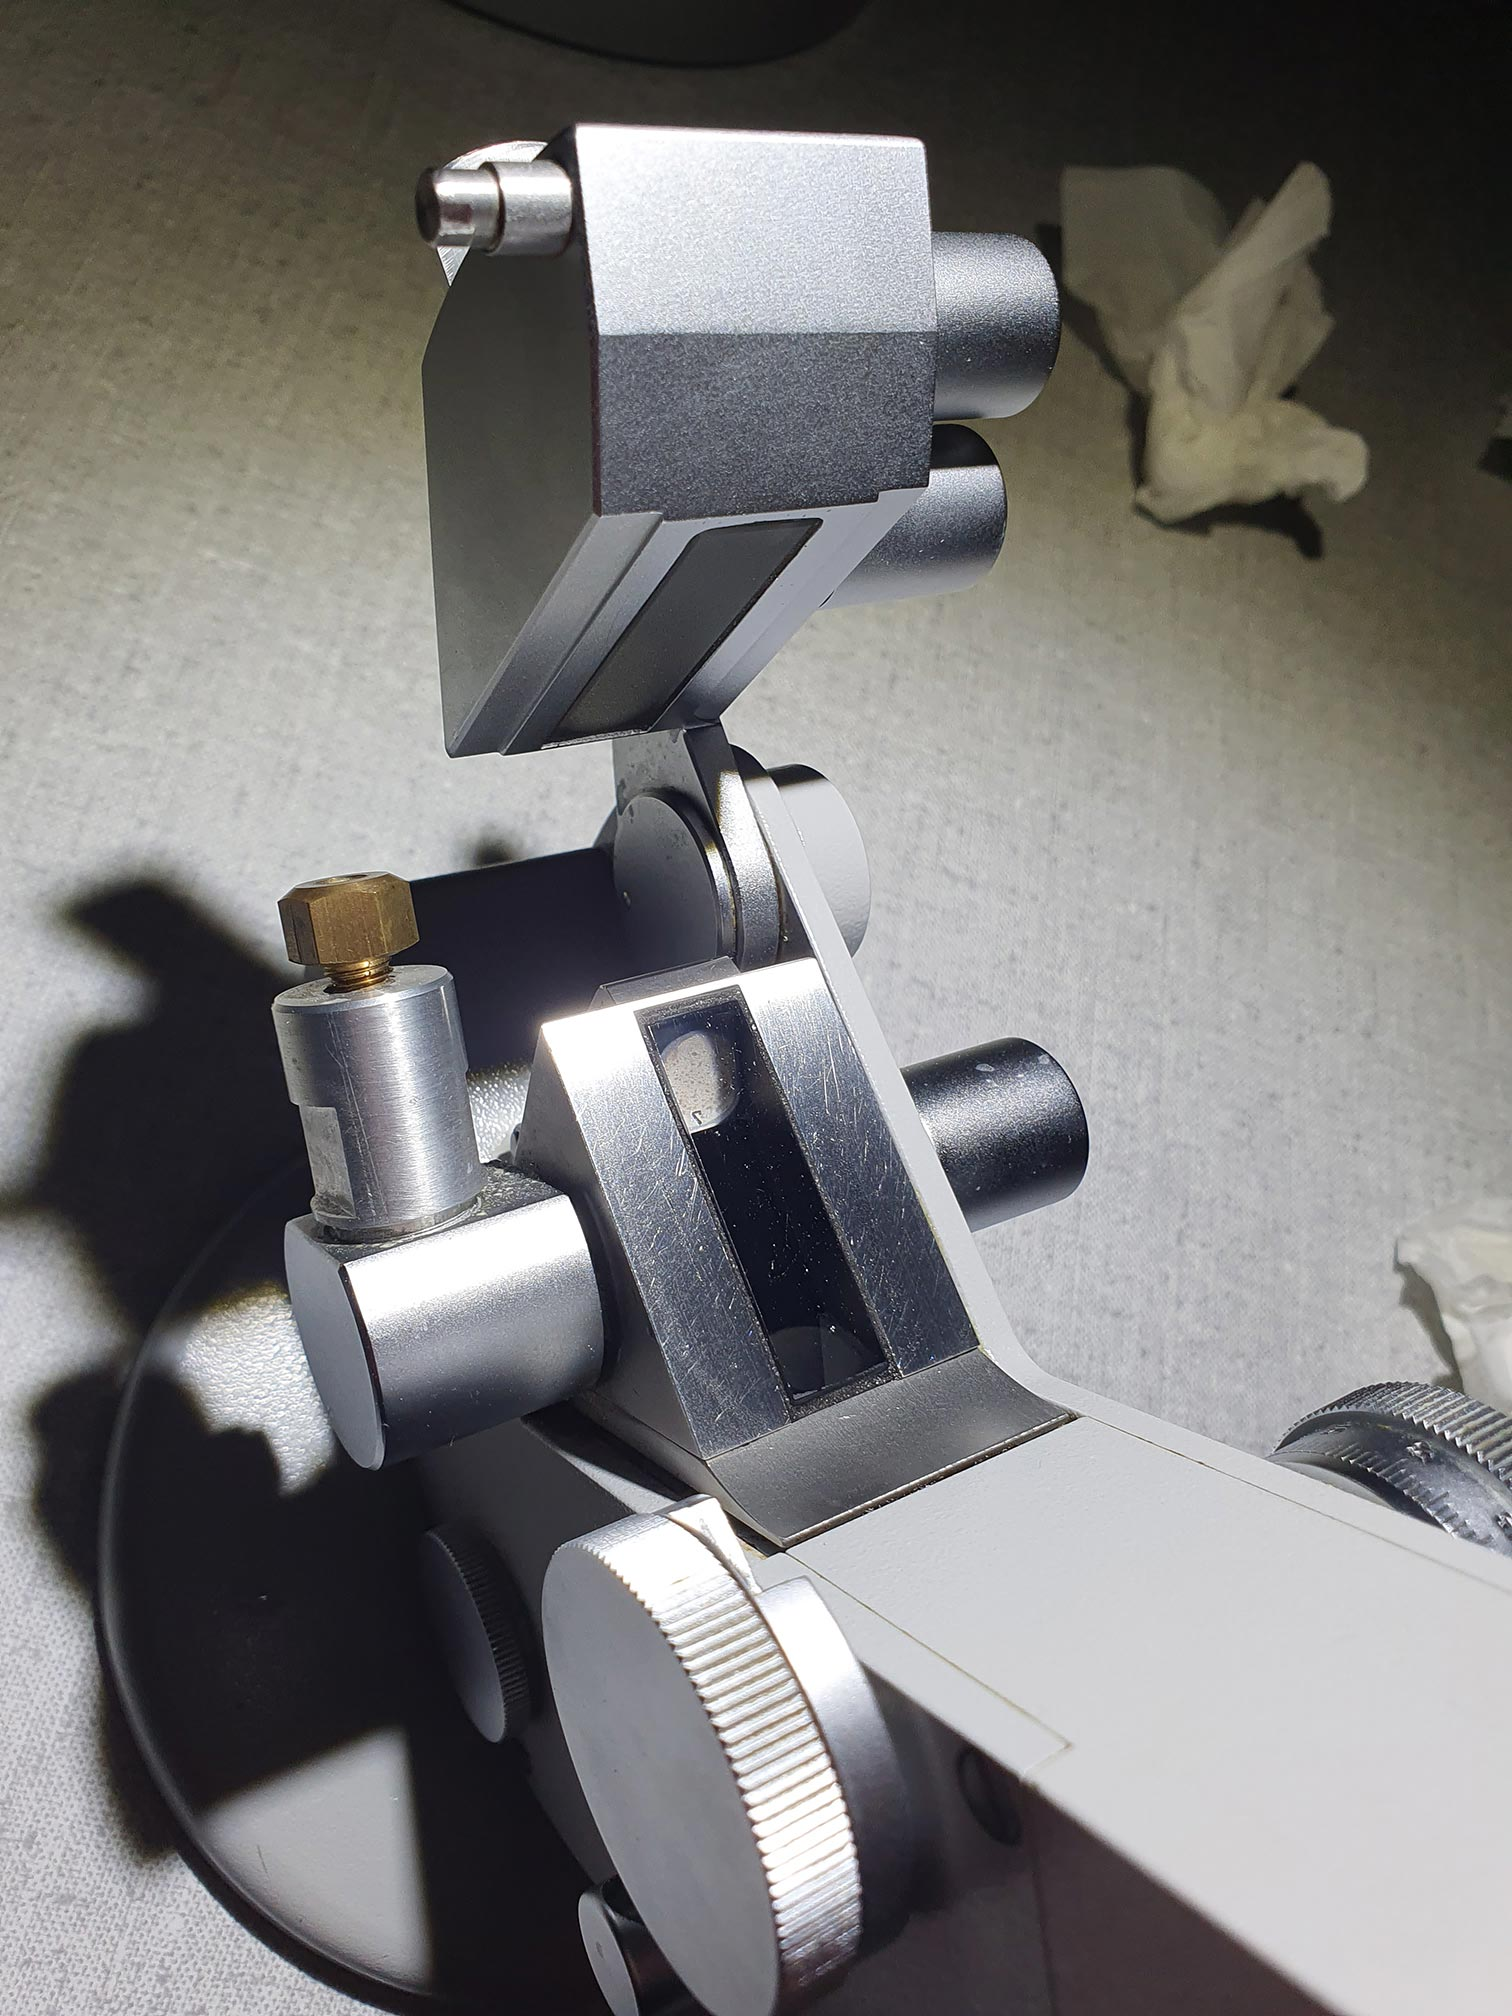
\includegraphics[width=0.4\linewidth]{nudes/abbe2.jpg}
    \caption{Aufbau des Versuches Abbe-Refraktometer (links). Beleuchtungsprisma ohne zu messender Flüssigkeit (rechts). }
    \label{fig:abbe}
\end{figure}



\section{Geräteliste} %jo holt a listn ------------------------------

    \begin{table}[H]
        \centering
        \caption{Im Versuch verwendete Geräte und Utensilien.}
        \label{tab:geraete}
        \begin{tabular}{| l | l | l |}
            \hline
            Gerät   & Gerätenummer  & Unsicherheit \\
            \hline
            Abbe-Refraktometer & {n.a} & {n.a} \\
            Reflexions-Refraktometer & {n.a} & {n.a} \\
            Laser & {n.a} & {n.a} \\
            Polarisator & Thorlabs CRM1/M & $\pm 2 deg. $ \\
            Halbkreisprisma & {n.a} & {n.a} \\
            Detektor & {n.a} & {n.a} \\
            Winkelmessgerät & {n.a} & $\pm 0.1 deg. $ \\
            Multimeter <120 mV & U3402A & $\pm 0.012 \% + 8 dig$ \cite{multimeter} \\
            Multimeter 120 - 1200 mV & U3402A & $\pm 0.012 \% + 5 dig$ \cite{multimeter} \\
            Wasser/Zucker Probe & {n.a} & {n.a}\\
            \hline
        \end{tabular}
    \end{table}


\section{Versuchsdurchführung \& Messergebnisse} %nachvollziehbar und klar dargestellt ------------------------------
Polarisator bei 110° p-Polarisiert und bei 200° s-Polarisiert. 
Bevor die Messungen beginnen, gilt es die Winkelskalen einzustellen. Dazu schließt man die Blende komplett, entfernt den Halbkreisprisma und richtet den Detektor zentral auf den Laser. 
Das ist die null-Position. Der Prisma wir wieder eingesetzt und so eingestellt, dass der reflektierte Strahl wieder zum Laser zurückreflektiert wird. Das ist die null-Position des Prismas. 
Zur überprüfung wird der Prisma auf 45.0° gedreht und der Detektor auf 90.0°. Der reflektierte Strahl sollte genau auf den Detektor fallen. 
Dies tut er jedoch nur bei einem Winkel von 90.7°, was bedeutet, dass die Messung eine Winkelunsicherheit von $\Delta \varphi \pm 0.7 deg. $ hat. 
\\
\\
Im ersten Teil mit dem Reflextions-Refraktometer wird der reflektierte Srahl einer Luft-Glas Grenzschicht gemessen. 
Zuvor wird jedoch noch der Brewsterwinkel bestimmt. Bei entfernten Prisma wird einmal für p-Polarisiertes und einmal für s-Polarisiertes Licht die Referenzspannung $U_0$ gemessen. Der Prisma wird wieder eingesetzt und 
durch schrittweises Drehen des Prismentisches wird der Einfallswinkel $\varphi_{Ein}$ verändert. Der Detektorwinkel $\varphi_D$ wird durch Drehen des Detektors bestimmt. Um genau die Mitte des Detektors zu treffen, 
wir die Blende geschlossen und der reflektierte Strahl auf die Mitte der Blende gerrichtet. Bei geöffneter Blende wird anschließend die reflektierte Spannung $U_R$ für einmal p-Polarisiertes und einmal für s-Polarisiertes Licht gemessen. 
Durch verdecken des Lasers wird die Detektorspannung $U_D$ gemessen. Dies wird insgesamt 15 mal wiederholt. 

\begin{table}[H]
    \centering
    \caption{Messergebnisse für eine Luft-Glas Grenzfläche bei p-Polarisiertem Licht. }
    \label{tab:mess luft glas p-pol}
    \begin{tabular}{| l | l | l | l | l | l |}
        \hline
        Nr. & $U_0 \pm 0.15 $ / mV & $U_D \pm 0.009$ / mV & $U_{R}$ / mV & $\varphi_{Ein} \pm 0.7$ / deg. & $\varphi_D \pm 0.7$ / deg.  \\
        \hline
        1  & 826.32 & -5.047 & 29.097 $\pm$ 0.012 & 15.0 & -147.8 \\
        2  & 826.32 & -5.184 & 15.378 $\pm$ 0.010 & 20.0 & -139.2 \\
        3  & 826.32 & -5.396 & 13.262 $\pm$ 0.010 & 25.0 & -128.0 \\
        4  & 826.32 & -5.594 & 10.798 $\pm$ 0.010 & 30.0 & -119.7 \\
        5  & 826.32 & -5.619 & 7.032  $\pm$ 0.009 & 35.0 & -109.4 \\
        6  & 826.32 & -5.863 & 3.184  $\pm$ 0.009 & 40.0 & -99.2  \\
        7  & 826.32 & -5.934 & -1.239 $\pm$ 0.008 & 45.0 & -87.9  \\
        8  & 826.32 & -5.932 & -4.141 $\pm$ 0.008 & 50.0 & -79.1  \\
        9  & 826.32 & -5.972 & -5.824 $\pm$ 0.008 & 55.0 & -68.5  \\
        10 & 826.32 & -5.962 & -4.574 $\pm$ 0.008 & 60.0 & -60.2  \\
        11 & 826.32 & -5.954 & 4.178  $\pm$ 0.009 & 65.0 & -49.8  \\
        12 & 826.32 & -5.905 & 26.375 $\pm$ 0.012 & 70.0 & -39.4  \\
        13 & 826.32 & -5.874 & 82.346 $\pm$ 0.018 & 75.0 & -28.7  \\
        14 & 826.32 & -5.874 & 183.75 $\pm$ 0.07 & 80.0 & -19.2  \\
        15 & 826.32 & -5.852 & 419.78 $\pm$ 0.10 & 85.0 & -8.2   \\
        \hline
    \end{tabular}
\end{table}

\begin{table}[H]
    \centering
    \caption{Messergebnisse für eine Luft-Glas Grenzfläche bei s-Polarisiertem Licht. }
    \label{tab:mess luft glas s-pol}
    \begin{tabular}{| l | l | l | l | l | l |}
        \hline
        Nr. & $U_0 \pm 0.12 $ / mV & $U_D \pm 0.009$ / mV & $U_{R}$ / mV & $\varphi_{Ein} \pm 0.7$ / deg. & $\varphi_D \pm 0.7$ / deg.  \\
        \hline
        1  & 555.54 & -5.047 & 14.638  $\pm$ 0.010 & 15.0 & -147.8 \\
        2  & 555.54 & -5.184 & 16.944  $\pm$ 0.011 & 20.0 & -139.2 \\
        3  & 555.54 & -5.396 & 17.215  $\pm$ 0.011 & 25.0 & -128.0 \\
        4  & 555.54 & -5.594 & 18.226  $\pm$ 0.011 & 30.0 & -119.7 \\
        5  & 555.54 & -5.619 & 22.588  $\pm$ 0.011 & 35.0 & -109.4 \\
        6  & 555.54 & -5.863 & 27.110  $\pm$ 0.012 & 40.0 & -99.2  \\
        7  & 555.54 & -5.934 & 37.612  $\pm$ 0.013 & 45.0 & -87.9  \\
        8  & 555.54 & -5.932 & 46.118  $\pm$ 0.014 & 50.0 & -79.1  \\
        9  & 555.54 & -5.972 & 58.697  $\pm$ 0.016 & 55.0 & -68.5  \\
        10 & 555.54 & -5.962 & 78.027  $\pm$ 0.018 & 60.0 & -60.2  \\
        11 & 555.54 & -5.954 & 100.634 $\pm$ 0.020 & 65.0 & -49.8  \\
        12 & 555.54 & -5.905 & 136.88  $\pm$ 0.07 & 70.0 & -39.4  \\
        13 & 555.54 & -5.874 & 208.06  $\pm$ 0.08 & 75.0 & -28.7  \\
        14 & 555.54 & -5.874 & 280.71  $\pm$ 0.09 & 80.0 & -19.2  \\
        15 & 555.54 & -5.852 & 392.42  $\pm$ 0.10 & 85.0 & -8.2   \\
        \hline
    \end{tabular}
\end{table}

\noindent
Für eine Glas-Luft Grenzfläche wird der Versuch wiederholt. Dazu dreht man den Prismentisch auf 180°, dreht den Prisma um und somit hat man eine neue null-Position. 

\begin{table}[H]
    \centering
    \caption{Messergebnisse für eine Glas-Luft Grenzfläche bei p-Polarisiertem Licht. }
    \label{tab:mess glas luft p-pol}
    \begin{tabular}{| l | l | l | l | l | l |}
        \hline
        Nr. & $U_0 \pm 0.15 $ / mV & $U_D \pm 0.009$ / mV & $U_{R}$ / mV & $\varphi_{Ein} \pm 0.7$ / deg. & $\varphi_D \pm 0.7$ / deg.  \\
        \hline
        1  & 826.32 & -5.425 & 10.268 $\pm$ 0.010 & 15.0 & -148.6 \\
        2  & 826.32 & -5.359 & 6.894  $\pm$ 0.009 & 20.0 & -139.1 \\
        3  & 826.32 & -5.511 & 1.776  $\pm$ 0.009 & 25.0 & -128.1 \\
        4  & 826.32 & -5.543 & -2.431 $\pm$ 0.008 & 30.0 & -120.5 \\
        5  & 826.32 & -5.719 & -0.478 $\pm$ 0.008 & 35.0 & -110.0 \\
        6  & 826.32 & -5.789 & 36.692 $\pm$ 0.013 & 40.0 & -99.8  \\
        7  & 826.32 & -5.936 & 519.59 $\pm$ 0.12 & 45.0 & -88.7  \\
        8  & 826.32 & -5.908 & 510.97 $\pm$ 0.12 & 55.0 & -68.4  \\
        10 & 826.32 & -5.955 & 557.28 $\pm$ 0.12 & 60.0 & -60.4  \\
        11 & 826.32 & -5.963 & 589.87 $\pm$ 0.13 & 65.0 & -50.1  \\
        12 & 826.32 & -5.915 & 638.36 $\pm$ 0.13 & 70.0 & -39.8  \\
        13 & 826.32 & -5.832 & 668.14 $\pm$ 0.14 & 75.0 & -29.1  \\
        14 & 826.32 & -5.817 & 688.48 $\pm$ 0.14 & 80.0 & -19.4  \\
        15 & 826.32 & -5.879 & 700.82 $\pm$ 0.14 & 85.0 & -8.5   \\
        \hline
    \end{tabular}
\end{table}

\begin{table}[H]
    \centering
    \caption{Messergebnisse für eine Glas-Luft Grenzfläche bei s-Polarisiertem Licht. }
    \label{tab:mess glas luft s-pol}
    \begin{tabular}{| l | l | l | l | l | l |}
        \hline
        Nr. & $U_0 \pm 0.12 $ / mV & $U_D \pm 0.009$ / mV & $U_{R}$ / mV & $\varphi_{Ein} \pm 0.7$ / deg. & $\varphi_D \pm 0.7$ / deg.  \\
        \hline
        1  & 555.54 & -5.425 & 12.193  $\pm$ 0.010 & 15.0  & -148.6 \\
        2  & 555.54 & -5.359 & 16.648  $\pm$ 0.010& 20.0  & -139.1 \\
        3  & 555.54 & -5.511 & 21.414  $\pm$ 0.011 & 25.0  & -128.1 \\
        4  & 555.54 & -5.543 & 29.556  $\pm$ 0.012 & 30.0  & -120.5 \\
        5  & 555.54 & -5.719 & 55.858  $\pm$ 0.015 & 35.0  & -110.0 \\
        6  & 555.54 & -5.789 & 119.634 $\pm$ 0.023 & 40.0  & -99.8  \\
        7  & 555.54 & -5.936 & 367.57  $\pm$ 0.10 & 45.0  & -88.7  \\
        8  & 555.54 & -5.908 & 360.52  $\pm$ 0.10 & 50.0  & -79.5  \\
        9  & 555.54 & -5.915 & 346.67  $\pm$ 0.10 & 55.0  & -68.4  \\
        10 & 555.54 & -5.955 & 378.43  $\pm$ 0.10 & 60.0  & -60.4  \\
        11 & 555.54 & -5.963 & 388.25  $\pm$ 0.10 & 65.0 & -50.1  \\
        12 & 555.54 & -5.915 & 409.67  $\pm$ 0.10 & 70.0 & -39.8  \\
        13 & 555.54 & -5.832 & 427.86  $\pm$ 0.11 & 75.0 & -29.1  \\
        14 & 555.54 & -5.817 & 447.67  $\pm$ 0.11 & 80.0 & -19.4  \\
        15 & 555.54 & -5.879 & 482.37  $\pm$ 0.11 & 85.0 & -8.5   \\
        \hline
    \end{tabular}
\end{table}

\noindent
Im dritten Teil des Experimentes mit dem Reflexions-Refraktometer wird der brechende-Winkel einer Luft-Glas Grenzfläche bestimmt. 
Dazu wird der
\begin{table}[H]
    \centering
    \caption{winkel}
    \label{tab:3.3}
    \begin{tabular}{| l | l | l |}
        \hline
        Nr. &  $\varphi_{Ein} \pm 0.7$ / deg. & $\varphi_D \pm 0.7$ / deg.  \\
        \hline
        1   & 20.0  & -6.8  \\
        2   & 25.0  & -8.1  \\
        3   & 30.0  & -10.0 \\
        4   & 35.0  & -11.3 \\
        5   & 40.0  & -13.7 \\
        6   & 45.0  & -15.7 \\
        7   & 50.0  & -19.2 \\
        8   & 55.0  & -21.4 \\
        9   & 60.0  & -24.2 \\
        10  & 65.0  & -27.0 \\
        \hline
    \end{tabular}
\end{table}


\section{Auswertung und Unsicherheitsanalyse} %Nicht nur zahlen angeben ------------------------------

In der Auswertung werden zur erhöhten Genauigkeit durchgehend ungerundete Werte bis zu den Endergebnissen verwendet und nur zur Darstellung gerundet. \\
Zur Berechnung der Unsicherheiten wird, wenn nicht anders angegeben, die Größtunsicherheitsmethode verwendet.


\section{Diskussion} %diskussion der Unsicherheiten und Ergebnisse und evtl. verlgeich mit Literatur ------------------------------


\section{Zusammenfassung} %klare, übersichtliche vollständige beantwortung der Aufgabenstellung ------------------------------


\printbibliography[heading=bibintoc]
\end{document}
